\begin{figure}[H]
    \centering
    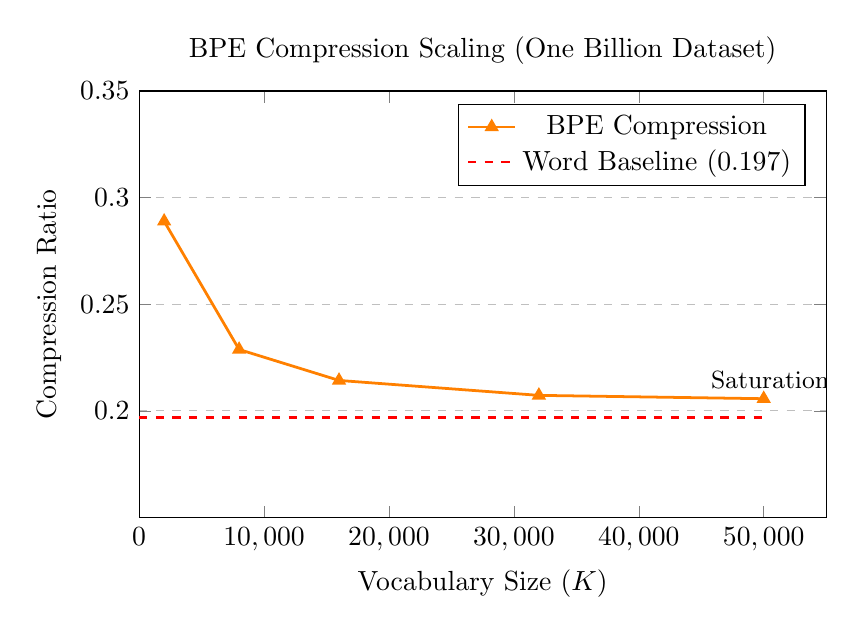
\begin{tikzpicture}
    \begin{axis}[
        title={BPE Compression Scaling (One Billion Dataset)},
        xlabel={Vocabulary Size ($K$)},
        ylabel={Compression Ratio},
        xmin=0, xmax=55000,
        ymin=0.15, ymax=0.35, 
        xtick={0, 10000, 20000, 30000, 40000, 50000},
        ytick={0, 0.20, 0.25, 0.30, 0.35},
        scaled x ticks=false,
        xticklabel style={
            /pgf/number format/fixed,
            /pgf/number format/1000 sep={,}
        },
        % ------------------------------------------
        legend pos=north east,
        ymajorgrids=true,
        grid style=dashed,
        width=0.85\textwidth,
        height=7cm,
    ]

    % BPE Compression Curve
    \addplot[
        color=orange,
        mark=triangle*,
        line width=1pt,
        ]
        coordinates {
        (2000, 0.2889)(8000, 0.2288)(16000, 0.2143)(32000, 0.2073)(50000, 0.20573)
        };
        \addlegendentry{BPE Compression}

    % Word-level Baseline Ratio
    \addplot[
        color=red,
        dashed,
        line width=1pt,
        domain=0:50000,
    ] {0.1968};
    \addlegendentry{Word Baseline (0.197)}

    % Saturation Point Label
    \node[anchor=south west] at (axis cs:45000, 0.20573) {\small Saturation};

    \end{axis}
    \end{tikzpicture}
    \caption{BPE Compression Ratio correlation with K = 2k, 4k, 8k, 16k, 32k, 50k. The graph illustrates how BPE approaches the theoretical maximum density of Word-level tokenization without the cost of OOV errors.}
    \label{fig:compression_one_billion}
\end{figure}